% !TeX spellcheck = en_US
%% 字体:方正静蕾简体
%%		 方正粗宋
\documentclass[a4paper,left=2.5cm,right=2.5cm,11pt]{article}
\usepackage[utf8]{inputenc}
\usepackage{fontspec}
\usepackage{cite}
\usepackage{xeCJK}
\usepackage{indentfirst}
\usepackage{titlesec}
\usepackage{longtable}
\usepackage{graphicx}
\usepackage{float}
\usepackage{rotating}
\usepackage{subfigure}
\usepackage{tabu}
\usepackage{amsmath}
\usepackage{setspace}
\usepackage{amsfonts}
\usepackage{appendix}
\usepackage{listings}
\usepackage{xcolor}
\usepackage{geometry}
\setcounter{secnumdepth}{4}
\usepackage{mhchem}
\usepackage{multirow}
\usepackage{extarrows}
\usepackage{hyperref}
\usepackage{caption}
\usepackage{color}

\titleformat*{\section}{\LARGE}
\renewcommand\refname{参考文献} %设置参考文献的形状
\renewcommand{\abstractname}{\sihao \cjkfzcs 摘{  }要}
%\titleformat{\chapter}{\centering\bfseries\huge\wryh}{}{0.7em}{}{}
%\titleformat{\section}{\LARGE\bf}{\thesection}{1em}{}{}
\titleformat{\subsection}{\Large\bfseries}{\thesubsection}{1em}{}{}
\titleformat{\subsubsection}{\large\bfseries}{\thesubsubsection}{1em}{}{}
\renewcommand{\contentsname}{{\cjkfzcs \centerline{目{  } 录}}}

\setCJKfamilyfont{cjkfzcs}{STSongti-SC-Regular}
% \setCJKfamilyfont{cjkhwxk}{STXingkai}
% \setCJKfamilyfont{cjkhwxk}{华文行楷}
% \setCJKfamilyfont{cjkfzcs}{方正粗宋简体}
\newcommand*{\cjkfzcs}{\CJKfamily{cjkfzcs}}
\newcommand*{\cjkhwxk}{\CJKfamily{cjkhwxk}}
% \newfontfamily\wryh{Microsoft YaHei}
% \newfontfamily\hwzs{STZhongsong}
\newfontfamily\hwst{STSong}
\newfontfamily\hwfs{STFangsong}
% \newfontfamily\jljt{MicrosoftYaHei}
% \newfontfamily\hwxk{STXingkai}
% \newfontfamily\hwzs{华文中宋}
% \newfontfamily\hwst{华文宋体}
% \newfontfamily\hwfs{华文仿宋}
% \newfontfamily\jljt{方正静蕾简体}
% \newfontfamily\hwxk{华文行楷}
\newcommand{\verylarge}{\fontsize{60pt}{\baselineskip}\selectfont}  
\newcommand{\chuhao}{\fontsize{44.9pt}{\baselineskip}\selectfont}  
\newcommand{\xiaochu}{\fontsize{38.5pt}{\baselineskip}\selectfont}  
\newcommand{\yihao}{\fontsize{27.8pt}{\baselineskip}\selectfont}  
\newcommand{\xiaoyi}{\fontsize{25.7pt}{\baselineskip}\selectfont}  
\newcommand{\erhao}{\fontsize{23.5pt}{\baselineskip}\selectfont}  
\newcommand{\xiaoerhao}{\fontsize{19.3pt}{\baselineskip}\selectfont} 
\newcommand{\sihao}{\fontsize{14pt}{\baselineskip}\selectfont}      % 字号设置  
\newcommand{\xiaosihao}{\fontsize{12pt}{\baselineskip}\selectfont}  % 字号设置  
\newcommand{\wuhao}{\fontsize{10.5pt}{\baselineskip}\selectfont}    % 字号设置  
\newcommand{\xiaowuhao}{\fontsize{9pt}{\baselineskip}\selectfont}   % 字号设置  
\newcommand{\liuhao}{\fontsize{7.875pt}{\baselineskip}\selectfont}  % 字号设置  
\newcommand{\qihao}{\fontsize{5.25pt}{\baselineskip}\selectfont}    % 字号设置 

\usepackage{diagbox}
\usepackage{multirow}
\boldmath
\XeTeXlinebreaklocale "zh"
\XeTeXlinebreakskip = 0pt plus 1pt minus 0.1pt
\definecolor{cred}{rgb}{0.8,0.8,0.8}
\definecolor{cgreen}{rgb}{0,0.3,0}
\definecolor{cpurple}{rgb}{0.5,0,0.35}
\definecolor{cdocblue}{rgb}{0,0,0.3}
\definecolor{cdark}{rgb}{0.95,1.0,1.0}
\lstset{   %设置代码的格式
	language=[x86masm]Assembler,
	numbers=left,
	numberstyle=\tiny\color{black},
	showspaces=false,
	showstringspaces=false,
	basicstyle=\scriptsize,
	keywordstyle=\color{purple},
	commentstyle=\itshape\color{cgreen},
	stringstyle=\color{blue},
	frame=lines,
	extendedchars=true, 
	xleftmargin=1em,
	xrightmargin=1em, 
	backgroundcolor=\color{cred},
	aboveskip=1em,
	breaklines=true,
	tabsize=4
} 

\newfontfamily{\monaco}{Monaco}
%\newfontfamily{\consolas}{Consolas}
%\setmonofont[Mapping={}]{Consolas}	%英文引号之类的正常显示,相当于设置英文字体
%\setsansfont{Consolas} %设置英文字体 Monaco, Consolas,  Fantasque Sans Mono
% \setCJKmainfont{华文中宋}
\setmainfont{Times New Roman}

\newcommand{\fic}[1]{\begin{figure}[H]
		\center
		\includegraphics[width=0.8\textwidth]{#1}
	\end{figure}}
	
\newcommand{\sizedfic}[2]{\begin{figure}[H]
		\center
		\includegraphics[width=#1\textwidth]{#2}
	\end{figure}}

\newcommand{\codefile}[1]{\lstinputlisting{#1}}


% 改变段间隔
\setlength{\parskip}{0.6em}
\linespread{1.1}
\usepackage{lastpage}
\usepackage{fancyhdr}
\pagestyle{fancy}

\lhead{\space \qquad \space}
\chead{homework3  \qquad Name:徐晓刚  \qquad Student ID:3140102480 \qquad}
\rhead{\qquad\thepage/\pageref{LastPage}}

\DeclareMathOperator\dif{d\!}


%设置双线页眉
\makeatletter                                         
\def\headrule{{\if@fancyplain\let\headrulewidth\plainheadrulewidth\fi%
		\hrule\@height 1.5pt \@width\headwidth\vskip1pt%上面线为1pt粗  
		\hrule\@height 0.5pt\@width\headwidth  %下面0.5pt粗            
		\vskip-2\headrulewidth\vskip-1.5pt}      %两条线的距离1pt      
	\renewcommand{\headrule}{\hrule depth0pt height0.15truemm width\textwidth}  
	\vspace{6mm}}     %双线与下面正文之间的垂直间距              
\makeatother  

\begin{document}
	
	%\clearpage
	%\thispagestyle{empty}
   \begin{longtable}{p{12cm}p{5cm}p{5cm}}
	%\begin{longtable}[位置]{列格式}
	%多行进行编写
	\multirow{6}{*}{ \xiaoerhao  \color{red}{Artificial intelligence}} \multirow{6}{*}{ \xiaoerhao Homework3 \space \space \space \space} & 专业:信息工程 \\
	& 姓名:徐晓刚 \\
	& 学院:信电学院 \\
	& 学号:3140102480 \\
	& 日期:\today \\
	& 地点:玉泉5舍 \\
\end{longtable}

\section*{Problem 1}
\subsection*{6.5}
In order to explain this cryptarithmetic problem, we will solve the problem based on back-tracking with forward checking and the MRV and least-constraining-value.
The constrain here including: to satisfy the equation, the variables T,W,O,F,U,R can not be repeat, F can not be zero.
So we can begin our algorithm as following:

\begin{itemize}
\item  \wuhao {\textbf{a.} We choose value for $C_3$, the domain is \{0,1\}}
\item \wuhao {\textbf{b.}Firstly, we choose value 1 for $C_3$,because F can not be zero and $F=C_3$}
\item \wuhao {\textbf{c.} Since $F=C_3$, so we choose $F=1$}
\item \wuhao {\textbf{d.}Now $C_2$ and $C_1$ are tied for minimum remaining values at 2. According to the principle of MRV. Now we choose $C_2$}
\item \wuhao {\textbf{e.}Since Either value will be survives forward checking and according to the principle of least-constraining-value, we can arbitrarily choose value 0 for $C_2$ }
\item \wuhao {\textbf{f.}Now we should choose $C_1$, we can also arbitrarily choose 0 for value of $C_1$}
\item \wuhao {\textbf{g.}We now choose for O. The variable O must be an even number since $T+T \% 10=O$, So we choose 4 as the value of O.}
\item \wuhao {\textbf{h.}Variable R now has only one remaining value, which is 8}
\item \wuhao {\textbf{i.}Variable T now has only one remaining value, $T + T \% 10 = O$}
\item \wuhao {\textbf{j.} Variable U must be an even number since $W+W = U$ . we choose the value of 6 for this. Unless it will repeat with the variable of F, O and R.}
\item \wuhao {\textbf{k.} The variable W can be choose as 3 only}
The over all equation can be show as:
\par
\centering
\begin{tabular}{ccccc}
    &	&7 &  3 & 4\\
	&+ &7 & 3  & 4\\
	\hline
	&=1 & 4& 6 &8
\end{tabular}
\end{itemize}

\section*{Problem 2}
\subsection*{6.8}
The problem can be draw as following at first:
\begin{figure}[ht]
\centering
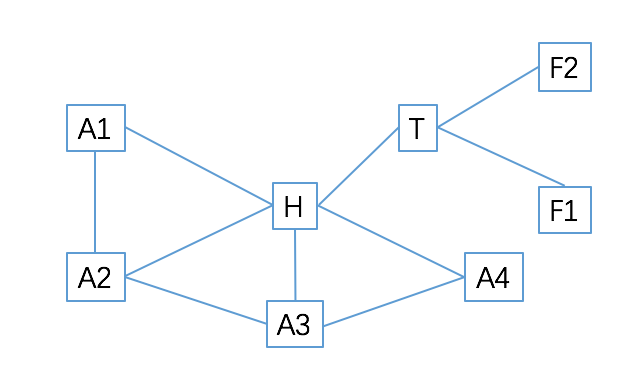
\includegraphics[width=10cm, height = 5cm]{figure1.png}  
\caption*{\small\it  The representation of this problem by figure. }
\end{figure}

We choose the variable order as A1, H, A4, F1, A2, F2, A3, T
We can set the value of $\{ R,G,B  \}$
The process can be explained as:
\begin{itemize}
	\item  \wuhao {\textbf{a.} A1 = R}
	\item \wuhao {\textbf{b.}  H =R, but it conflicts with A1}
	\item \wuhao {\textbf{c.}  H = G}
	\item \wuhao {\textbf{d.} A4 = R}
	\item \wuhao {\textbf{e.} F1 = R}
	\item \wuhao {\textbf{f.} A2 = R, but it conflicts with A1; A2 =G, but it will conflict with H, so A2 = B}
	\item \wuhao {\textbf{g.} F2 = R}
	\item \wuhao {\textbf{h.} A3 has no value to choose, so we must backtrack, the conflict set is \{A2, H, A4\} , so we jump to A2, and add \{ H, A4 \} to A2's conflict set }
	\item \wuhao {\textbf{i.} A2 has no value to choose, so we must backtrack, the conflict set is   \{ A1,H,A4 \}, so we jump to A4}
	\item \wuhao {\textbf{j.} A4 = B, F1 = R, A2 = B, F2 = R,A3 = R, T = B and we success at this step! }

\end{itemize}


\section*{Problem 3}
\subsection*{6.7}
This problem can be represented as a CSP by introducing a variable for each
color, pet, drink, country, and cigarette brand (a total of 25 variables). The value of each
variable is a number from 1 to 5 indicating the house's number.\par 
We can also solve this problem by Another representation is to have a tuple with five variables for each house, one with the domain of
 colors, one with pets, and so on. \par 

\sihao \textbf{Why we choose a representation while not another ? }  \par
We will consider two factors when choose the representation of a problem:
\begin{itemize}
	\item  It will be easy to represent all the constraints given in the problem definition.
	\item  The efficiency of finding a solution. 
\end{itemize}

Once the representation as be assured, we can choose the method of backtracking search  and MRV heuristic to solve this problem.

\sihao \textbf{The result }  \par
The result is zebra lives in the 5-th house, the people in the 1-st house drink water.


\begin{table}[!hbp]
	\centering
	\begin{tabular}{|c|c|c|c|c|c|}
		\hline
		\hline
		House & 1 & 2 & 3 & 4 & 5\\
		\hline
	    Color  &Yellow & Blue & Red &Lvory & Green \\
		\hline
	    Nationality & Norwegian & Ukrainian & Englishman & Spaniard & Japanese \\
		\hline
		Drink & \textbf{Water}  & Tea & Milk & Orange juice & Coffee\\
		\hline
		Candy & Kit Kats & Smarties& Snickers &Hershey Bar & Milky ways \\
		\hline  
		Pet & Fox & Horse & Snails & Dog & \textbf{Zebra} \\
		\hline
	\end{tabular}
	\caption*{Result of the problem}
\end{table} 


%\begin{figure}[ht]
%\centering
%\includegraphics[width=10cm]{pic3.png}  
%\caption*{\small\it Figure 10.4: 4个可能信息以及二值编码的例子}
%\end{figure}


%\begin{itemize}
%\item  \wuhao %{\color{red}{为了传送概率密度函数为$Pr(z)$的随机变量$z$,我们需要$-log_2Pr(z)$位信息}} %\par
%\end{itemize}

%\begin{quote}
%\centering {\color{red}{$length=constant + log\sigma + \frac{(y-\theta)^2}{\sigma^2} + %\frac{\theta^2}{2} \qquad(7.45)$}}
%\end{quote}

\end{document}

